\documentclass[a4paper, 11px]{article}

\usepackage[french]{babel}
\usepackage[utf8]{inputenc}
\usepackage{fancyhdr}
\usepackage{lastpage}
\usepackage{graphicx}
\usepackage{rotating}
\usepackage{textcomp}
\usepackage{xspace}
\usepackage[toc,page]{appendix}
\usepackage{array}
\usepackage{amssymb}
\usepackage{enumerate}
\usepackage{enumitem}
\usepackage{eso-pic}

% \usepackage{needspace}


%%%%%%
 
\usepackage{listings}

\lstset{
  morekeywords={},
  sensitive=f,
  morecomment=[l]--,
  morestring=[d]",
  showstringspaces=false,
  basicstyle=\small\ttfamily,
  keywordstyle=\bf\small,
  commentstyle=\itshape,
  stringstyle=\sf,
  extendedchars=true,
  columns=[c]fixed
}

% CI-DESSOUS: conversion des caractères accentués UTF-8 
% en caractères TeX dans les listings...
\lstset{
  literate=%
  {À}{{\`A}}1 {Â}{{\^A}}1 {Ç}{{\c{C}}}1%
  {à}{{\`a}}1 {â}{{\^a}}1 {ç}{{\c{c}}}1%
  {É}{{\'E}}1 {È}{{\`E}}1 {Ê}{{\^E}}1 {Ë}{{\"E}}1% 
  {é}{{\'e}}1 {è}{{\`e}}1 {ê}{{\^e}}1 {ë}{{\"e}}1%
  {Ï}{{\"I}}1 {Î}{{\^I}}1 {Ô}{{\^O}}1%
  {ï}{{\"i}}1 {î}{{\^i}}1 {ô}{{\^o}}1%
  {Ù}{{\`U}}1 {Û}{{\^U}}1 {Ü}{{\"U}}1%
  {ù}{{\`u}}1 {û}{{\^u}}1 {ü}{{\"u}}1%
}

%%%%%%%%%%
% TAILLE DES PAGES (A4 serré)

\setlength{\parindent}{1cm}
\setlength{\parskip}{1ex}
\setlength{\textwidth}{17cm}
\setlength{\textheight}{22,7cm}
\setlength{\oddsidemargin}{-.7cm}
\setlength{\evensidemargin}{-.7cm}


\renewcommand{\labelenumi}{\arabic{enumi}.} 
\renewcommand{\labelenumii}{\arabic{enumi}.\arabic{enumii}}
\renewcommand{\labelenumiii}{\arabic{enumi}.\arabic{enumii}.\arabic{enumiii}}

%%%%%%%%%%

\newcommand\BackgroundPic{
\put(0,0){
\parbox[b][\paperheight]{\paperwidth}{%
\vfill

\includegraphics[width=\paperwidth,height=\paperheight,
keepaspectratio]{background.jpg}%
\vfill
}}}
%%%%%%%

\begin{document}

\AddToShipoutPicture{\BackgroundPic}


\renewcommand{\appendixtocname}{Annexes}
\DeclareGraphicsExtensions{.pdf,.png,.jpg}

\begin{titlepage}
\setlength{\parindent}{0cm}

\begin{center}

% Upper part of the page
\begin{figure}[!h]

\includegraphics[bb=-550 -10 -250 20, scale=0.7]{./logo.pdf}
\end{figure}
% logo.pdf: 612x792 pixel, 72dpi, 21.59x27.94 cm, bb=0 0 612 792


\vspace{4cm}
\rule{\linewidth}{.5pt}
\vspace{2mm}


\begin{center}
{\LARGE GRAND CERCLE MOBILE - GCM}

\vspace{1cm}


{\Huge \bf Spécifications Externes}


\end{center}


\vspace{1cm}

%===================================================================
\begin{center}
$ $\\
\large{ \textbf{Luiza CICONE - Jérémy KREIN - Jérémy LUQUET - Paul MAYER}}\\
\large{ \textbf{ISI - IF}}
$ $\\
\end{center}
\rule{\linewidth}{.5pt}


\vfill

% Bottom of the page

{\large Mai 2012}

\end{center}
\end{titlepage}

\tableofcontents

\newpage

\section{Cas d'utilisations}
\begin{figure}[h!]
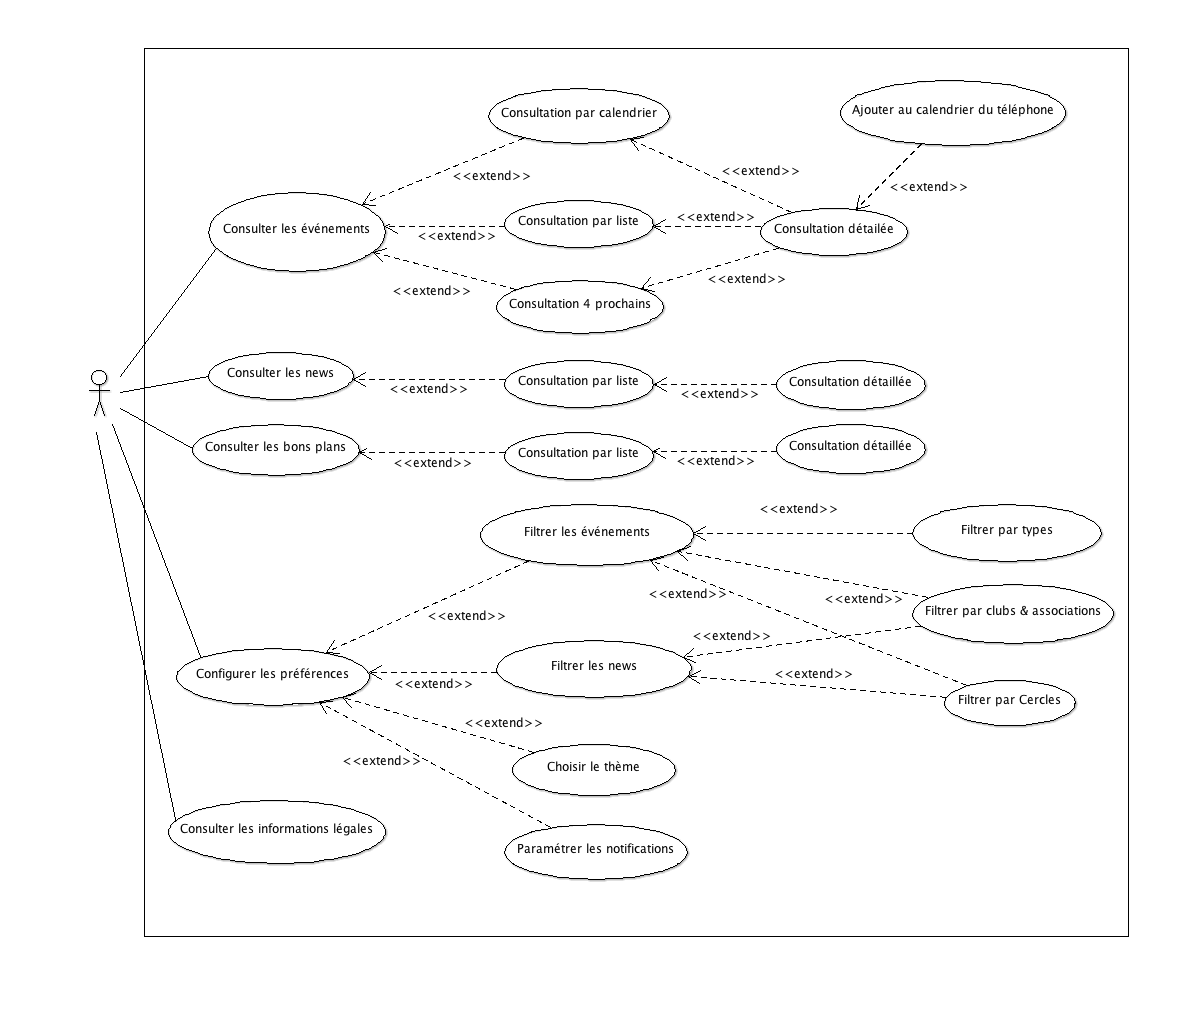
\includegraphics[width=20cm,height=15cm]{cas_utilisation.png}
\end{figure}

\newpage

\section{Modèle de tâches}
\vfill
\subsection{Fonctionnalités principales}
\begin{figure}[h!]
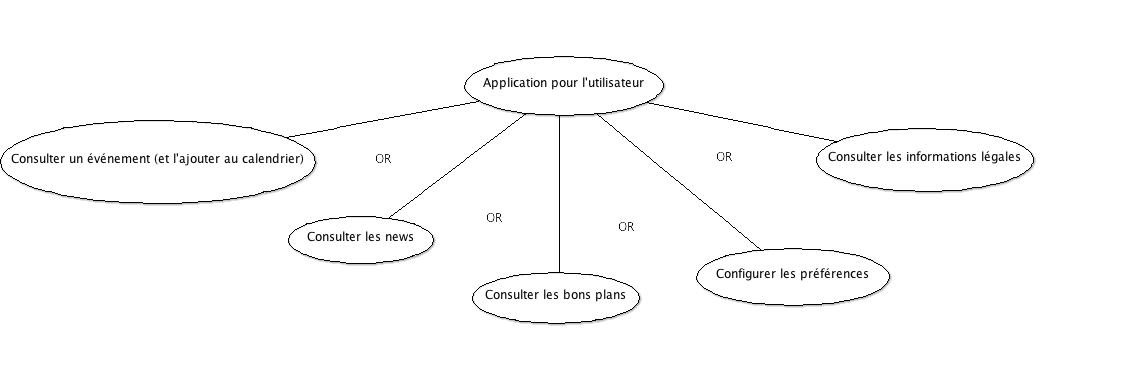
\includegraphics[width=18cm,height=6cm]{taches_generales.png}
\end{figure}

\subsection{Consulter les événements}
\begin{figure}[h!]
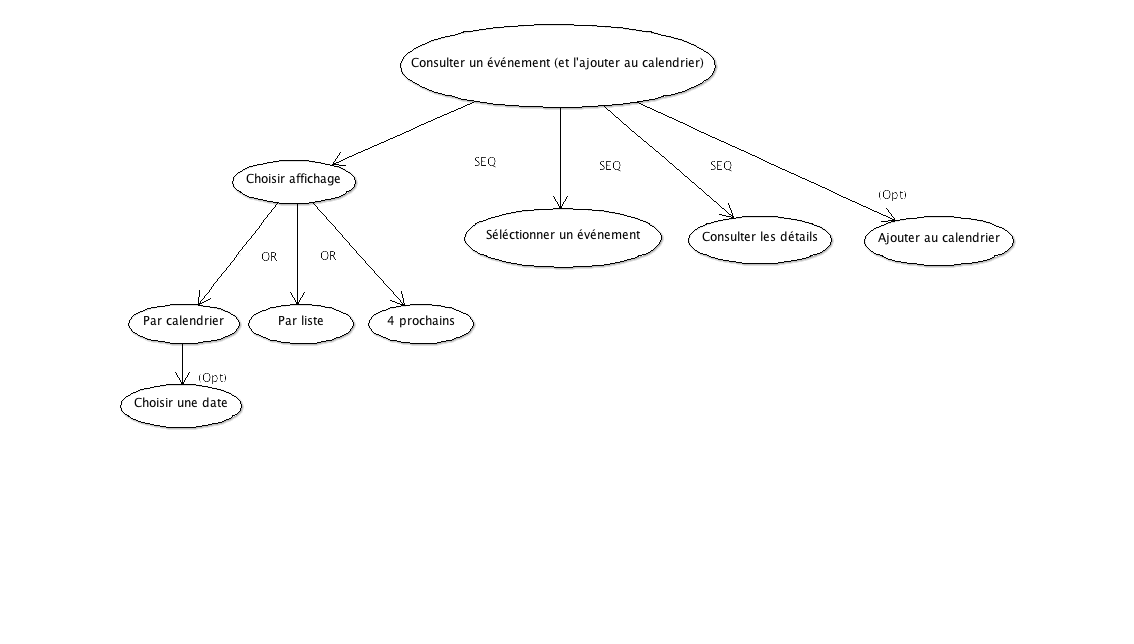
\includegraphics[width=20cm,height=11cm]{consulter_evenements.png}
\end{figure}
\vfill
\clearpage

\subsubsection{Ajouter au calendrier pour iOS}
\vfill
\begin{figure}[h!]
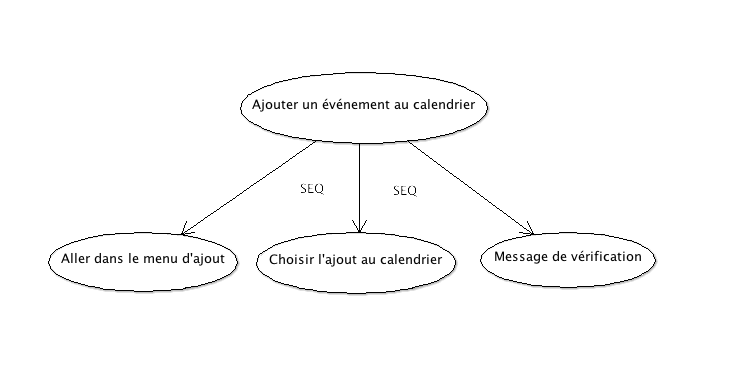
\includegraphics[width=18cm,height=8cm]{ajouter_evenement_calendrier_iOS.png}
\end{figure}

\subsubsection{Ajouter au calendrier pour Android}

\begin{figure}[h!]
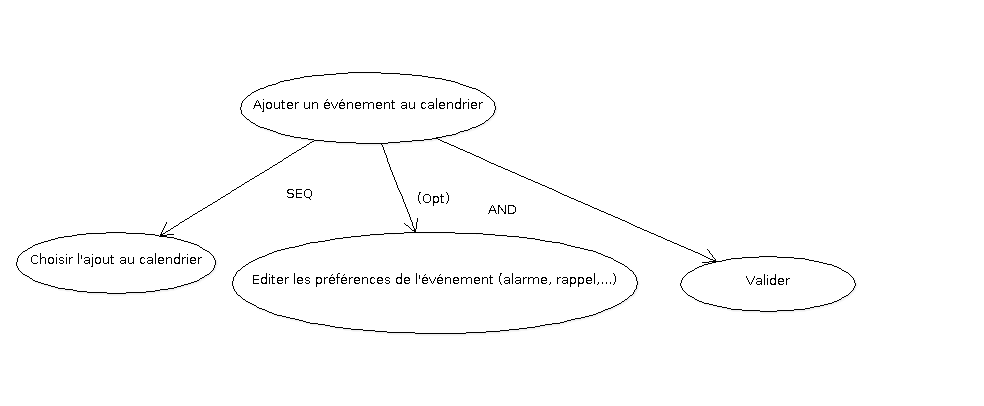
\includegraphics[width=18cm,height=8cm]{ajouter_evenement_calendrier_Android.png}
\end{figure}
\vfill
\clearpage

\subsection{Consulter une news}
\vfill
\begin{figure}[h!]
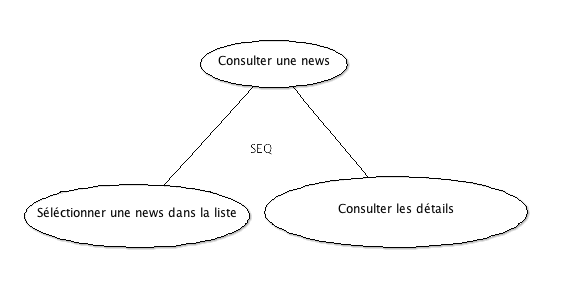
\includegraphics[width=18cm,height=8cm]{consulter_news.png}
\end{figure}

\subsection{Consulter un bon plan}

\begin{figure}[h!]
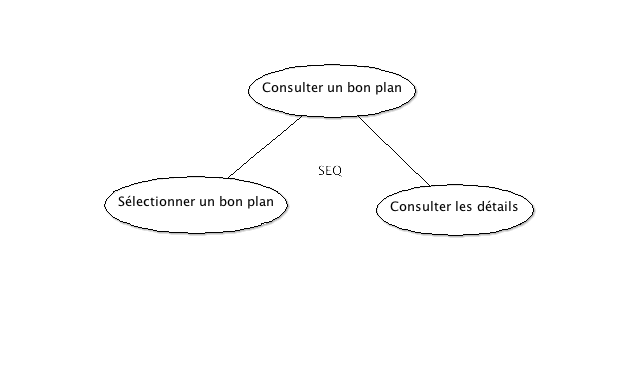
\includegraphics[width=18cm,height=8cm]{consulter_bonplans.png}
\end{figure}

\vfill
\clearpage
\subsection{Configurer les préférences}
\begin{figure}[h]
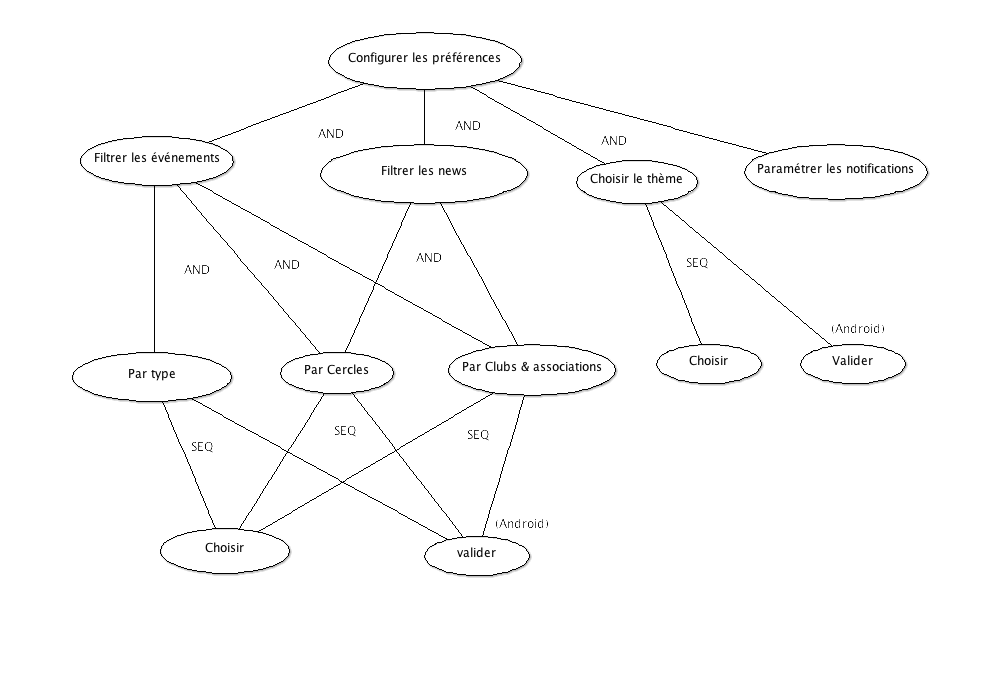
\includegraphics[width = \textwidth]{configurer_preferences.png}
\end{figure}
\vfill
\clearpage

\section{Diagrammes UML}
\begin{figure}[h]
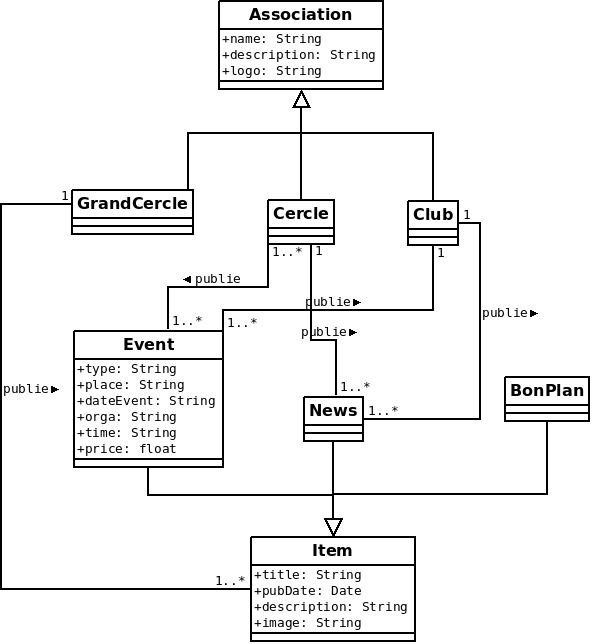
\includegraphics[width = 12cm,height=10cm]{classes.png}
\end{figure}
\vfill
\clearpage

\section{Interface utilisateur abstraite}
\subsection{Principale}
\vfill
\begin{figure}[h!]
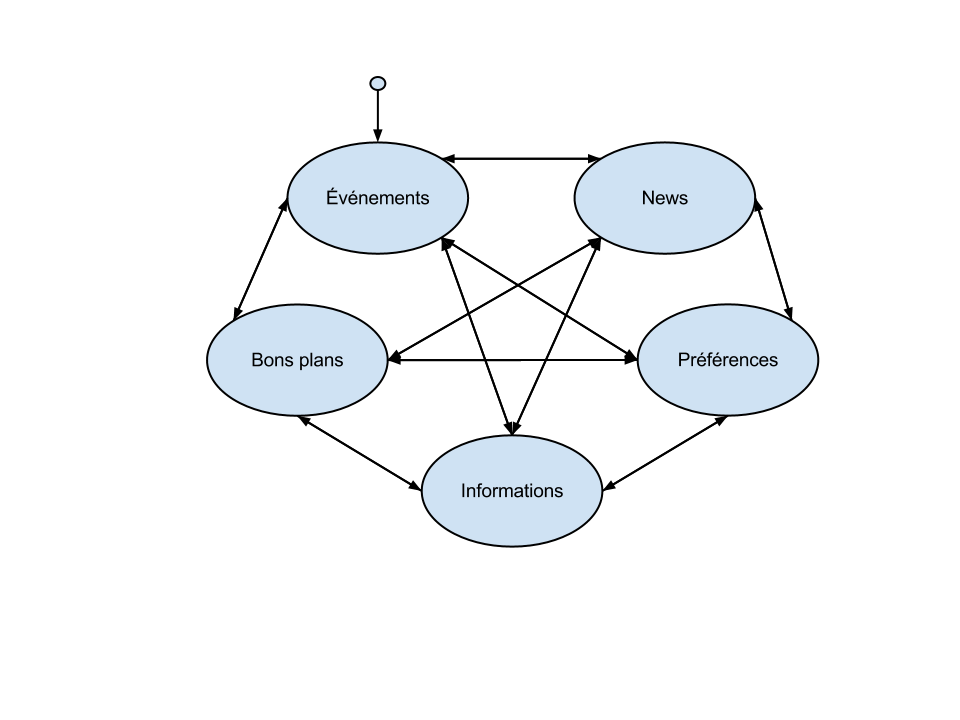
\includegraphics[width=18cm,height=8cm]{IUAprincipale.png}
\end{figure}

\subsection{Événements}
\vfill
\begin{figure}[h!]
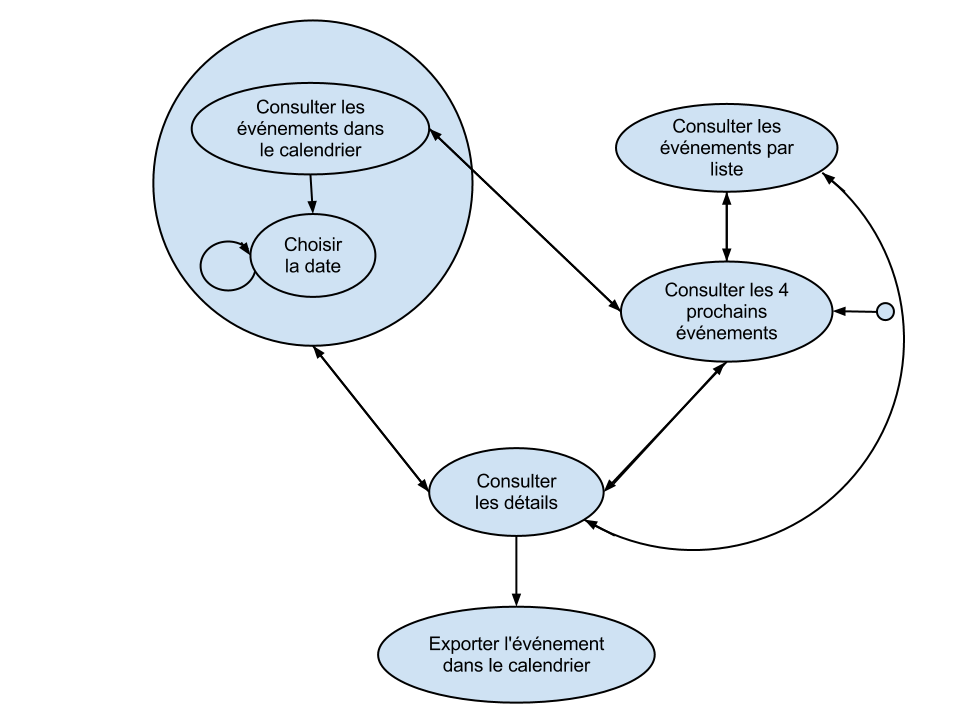
\includegraphics[width=18cm,height=8cm]{IUAevenements.png}
\end{figure}
\clearpage
\subsection{Bons plans et News}

\begin{figure}[h!]
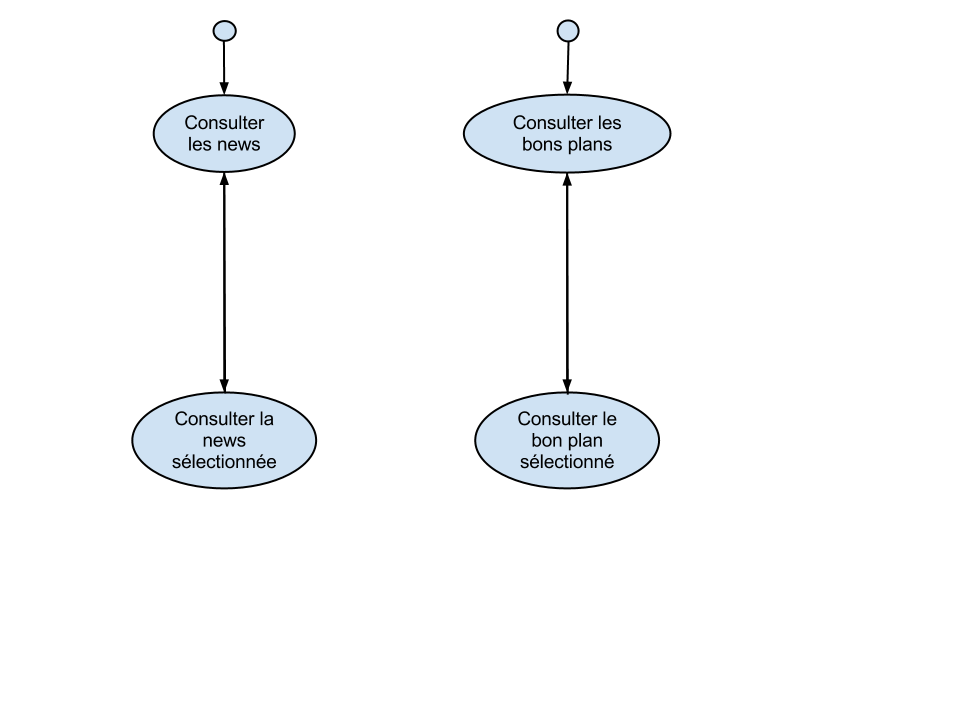
\includegraphics[width=18cm,height=8cm]{IUAnewsbonsplans.png}
\end{figure}

\subsection{Préférences}
\begin{figure}[h!]
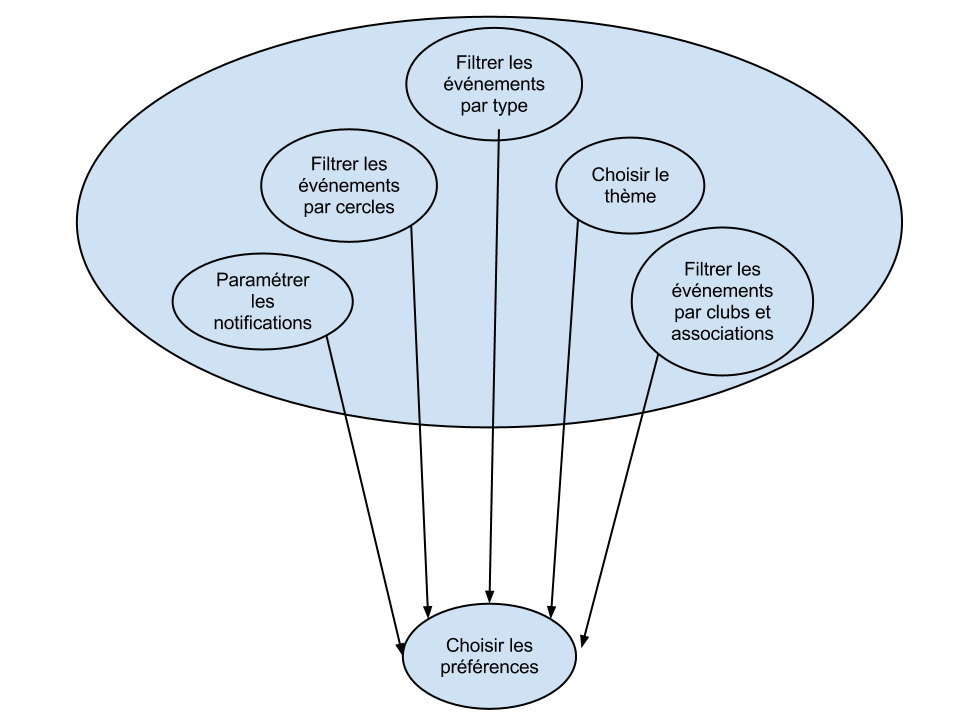
\includegraphics[width=18cm,height=8cm]{IUApreferences.png}
\end{figure}
\newpage

\section{Sketching}

\subsection{Sketching pour l'application iOS}
\subsubsection{Pages événements}
\vfill
\begin{figure}[htbp]
	\begin{minipage}[c]{.50\linewidth}
		\begin{center}
			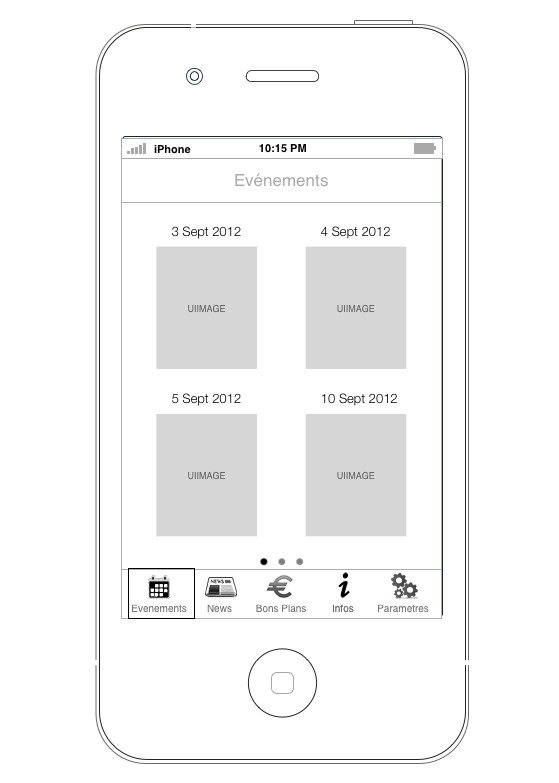
\includegraphics[scale=0.3]{../../Sketch/iOS/evenements_4_prochains.png}
		\end{center}
	\end{minipage}
	\hfill
	\begin{minipage}[c]{.50\linewidth}
		\begin{center}
			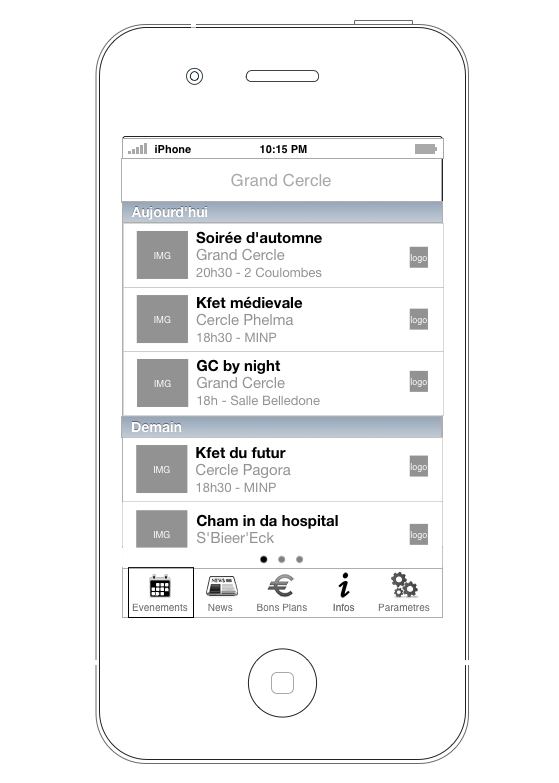
\includegraphics[scale=0.3]{../../Sketch/iOS/evenements_liste.png}
		\end{center}
	\end{minipage}
\end{figure}


\begin{figure}[htbp]
	\begin{minipage}[c]{.50\linewidth}
		\begin{center}
			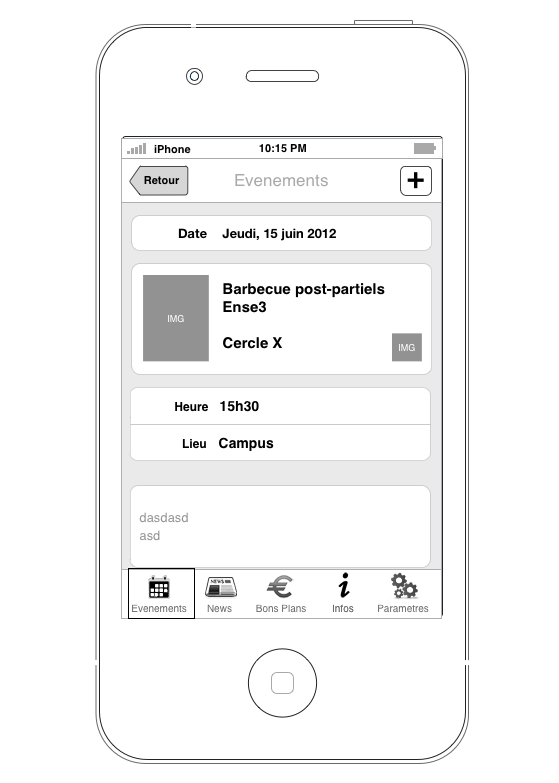
\includegraphics[scale=0.3]{../../Sketch/iOS/evenements_detail.png}
		\end{center}
	\end{minipage}
	\hfill
	\begin{minipage}[c]{.50\linewidth}
		\begin{center}
			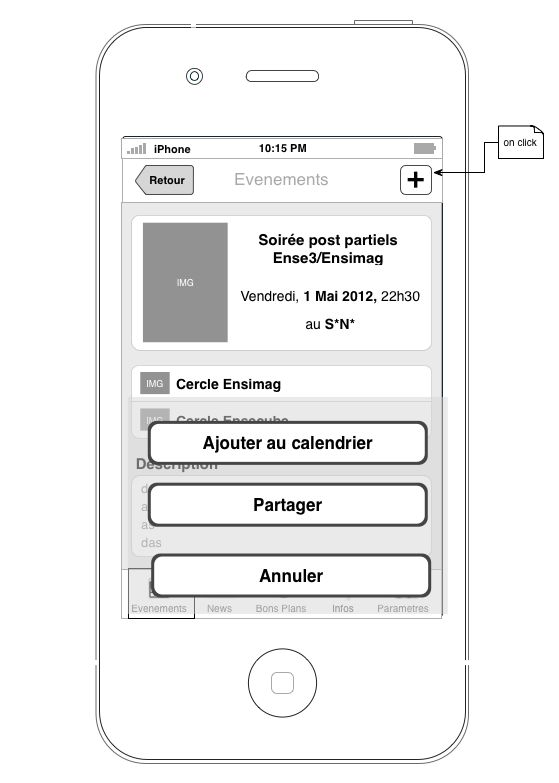
\includegraphics[scale=0.3]{../../Sketch/iOS/evenements_detail_plus.png}
		\end{center}
	\end{minipage}
\end{figure}
\vfill
\clearpage

\vfill
\subsubsection{Pages news}
\begin{figure}[htbp]
	\begin{minipage}[c]{.50\linewidth}
		\begin{center}
			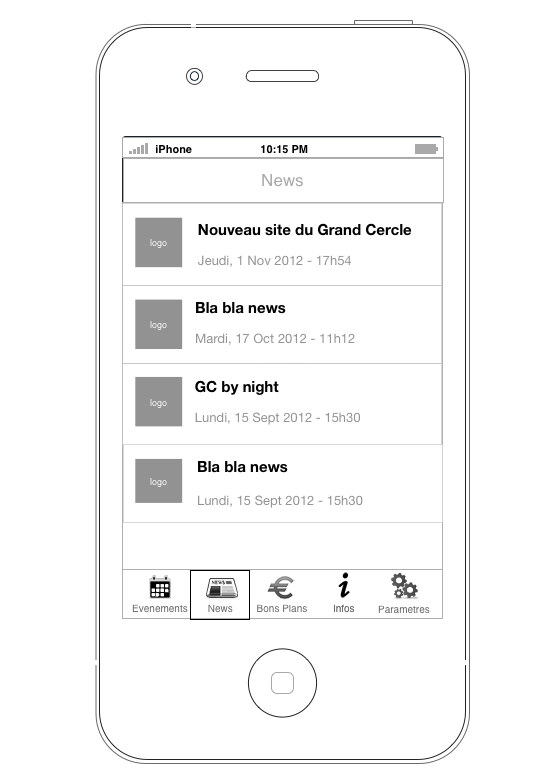
\includegraphics[scale=0.3]{../../Sketch/iOS/news_liste.png}
		\end{center}
	\end{minipage}
	\hfill
	\begin{minipage}[c]{.50\linewidth}
		\begin{center}
			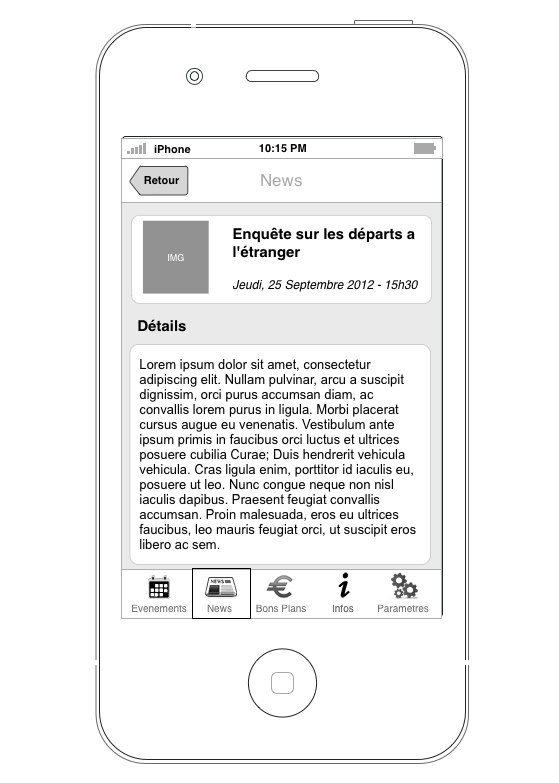
\includegraphics[scale=0.3]{../../Sketch/iOS/news_detail.png}
		\end{center}
	\end{minipage}
\end{figure}

\subsubsection{Pages bons plans}
\begin{figure}[htbp]
	\begin{minipage}[c]{.50\linewidth}
		\begin{center}
			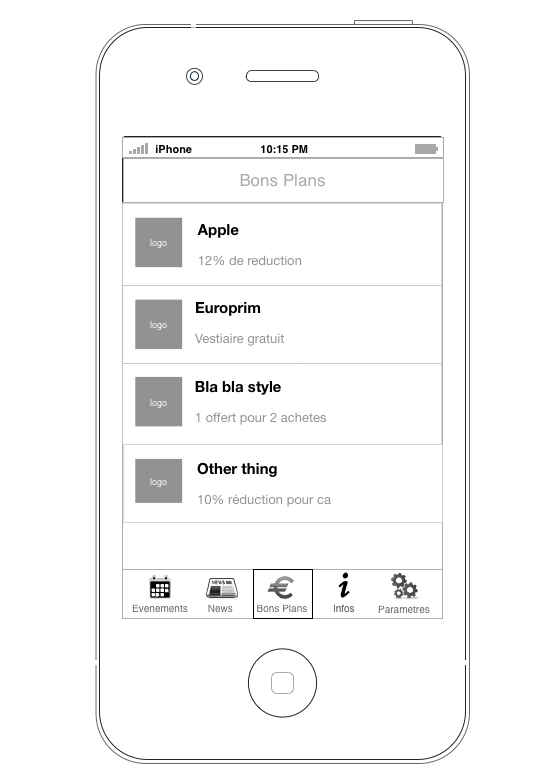
\includegraphics[scale=0.3]{../../Sketch/iOS/bons_plans_liste.png}
		\end{center}
	\end{minipage}
	\hfill
	\begin{minipage}[c]{.50\linewidth}
		\begin{center}
			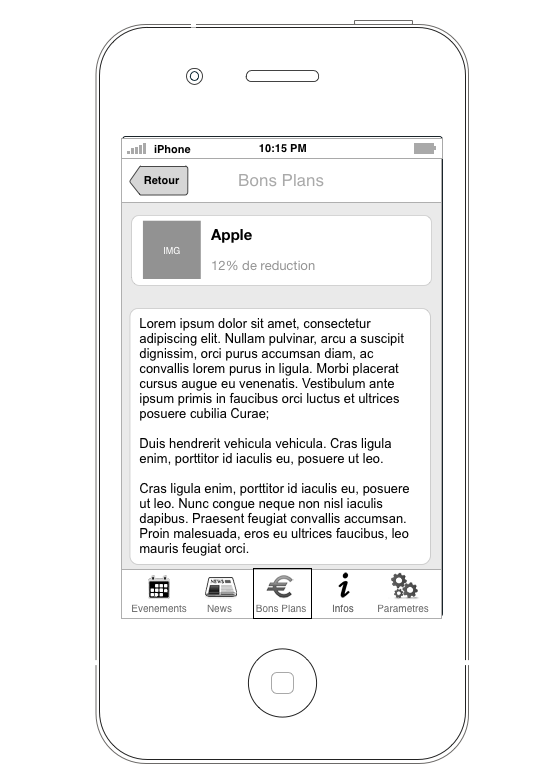
\includegraphics[scale=0.3]{../../Sketch/iOS/bons_plans_detail.png}
		\end{center}
	\end{minipage}
\end{figure}

\vfill
\clearpage

\subsubsection{Page informations}
\vfill
\begin{figure}[htbp]
	\begin{minipage}[c]{.50\linewidth}
		\begin{center}
			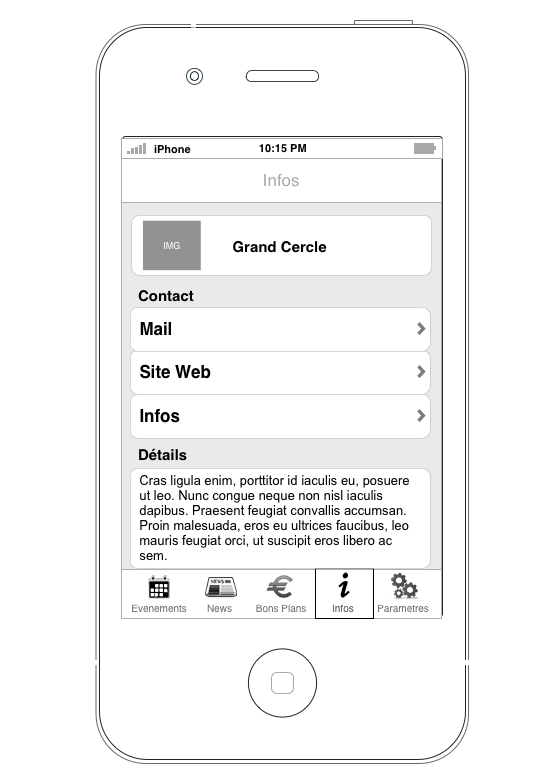
\includegraphics[scale=0.3]{../../Sketch/iOS/infos.png}
		\end{center}
	\end{minipage}
\end{figure}

\subsubsection{Pages paramètres}

En ce qui concerne les préférences utilisateurs, tous les choix se feront par le biais de checkbox comme pour l'application Android mais il n'y aura pas de boutton pour valider les choix effectués par les utilisateurs. 
En effet, les choix de thème seront pris en compte immédiatement après le "check" et les choix de filtre seront pris en compte quand l'utilisateur sortira de la page courante où il formule ses choix.
\begin{figure}[htbp]
	\begin{minipage}[c]{.50\linewidth}
		\begin{center}
			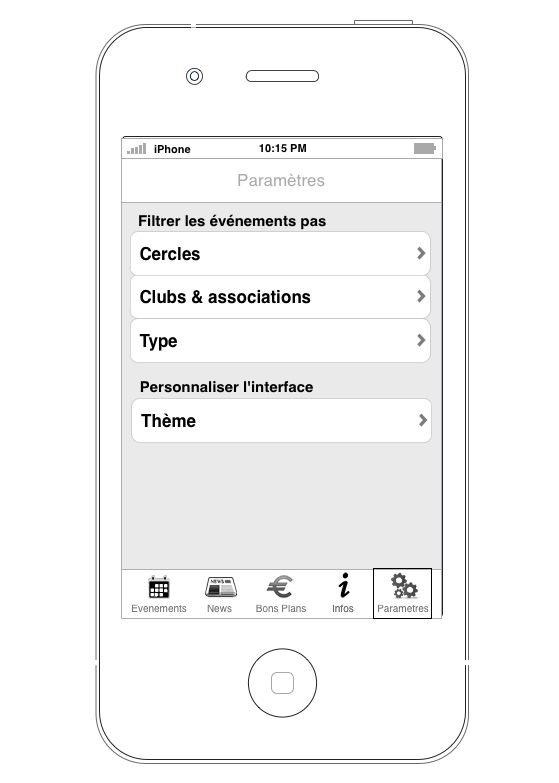
\includegraphics[scale=0.3]{../../Sketch/iOS/parametres.png}
		\end{center}
	\end{minipage}
	\hfill
	\begin{minipage}[c]{.50\linewidth}
		\begin{center}
			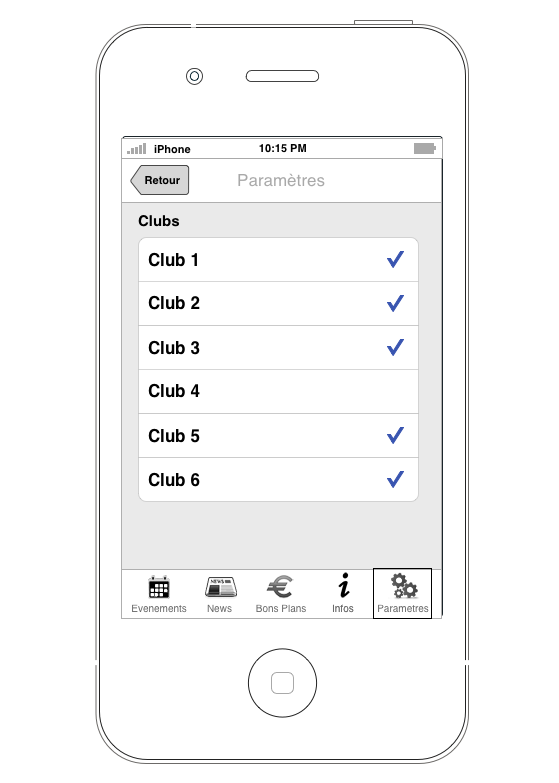
\includegraphics[scale=0.3]{../../Sketch/iOS/parametres_detail.png}
		\end{center}
	\end{minipage}
\end{figure}
\vfill
\clearpage


\subsection{Sketching pour l'application Android}
Les sketching de l'application Android ont été réalisés avec un plugin d'eclipse, \textbf{Wireframe Sketcher}, qui ne permet pas de séléctionner des onglets différents. Ainsi, dans toutes les pages présentées ci-après, l'onglet qui est mis en relief est toujours l'onglet "Evénements", ce qui ne représente pas toujours l'onglet actif. Afin de régler ce problème, l'onglet actif a été mis en gras.
\subsubsection{Pages événements}
\vfill
\begin{figure}[htbp]
	\begin{minipage}[c]{.50\linewidth}
		\begin{center}
			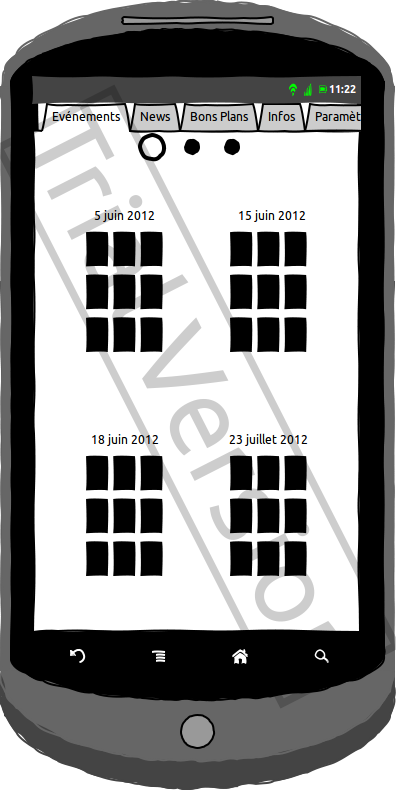
\includegraphics[scale=0.3]{../../Sketch/Android/quatreEvent.png}
		\end{center}
	\end{minipage}
	\hfill
	\begin{minipage}[c]{.50\linewidth}
		\begin{center}
			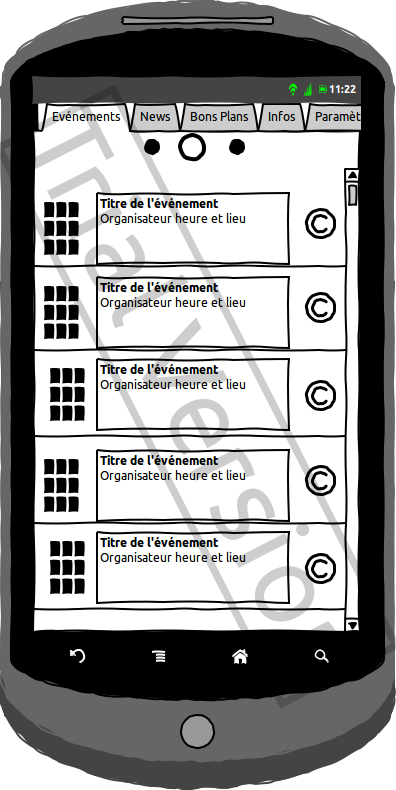
\includegraphics[scale=0.3]{../../Sketch/Android/ListEvent.png}
		\end{center}
	\end{minipage}
\end{figure}

\begin{figure}[htbp]
	\begin{minipage}[c]{.50\linewidth}
		\begin{center}
			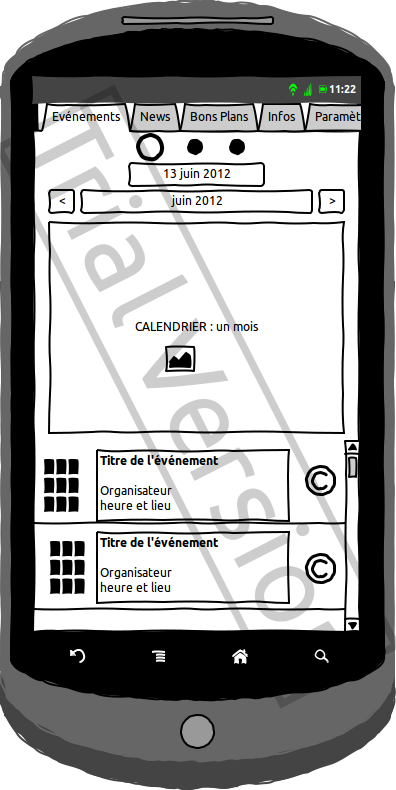
\includegraphics[scale=0.3]{../../Sketch/Android/Calendrier.png}
		\end{center}
	\end{minipage}
	\hfill
	\begin{minipage}[c]{.50\linewidth}
		\begin{center}
			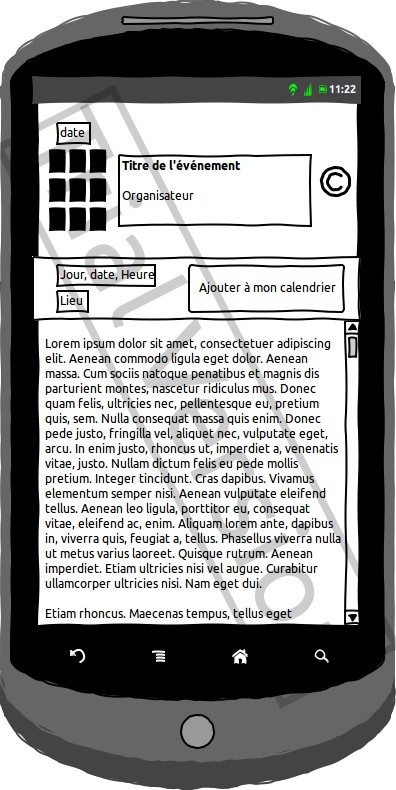
\includegraphics[scale=0.3]{../../Sketch/Android/DescrEvent.png}
		\end{center}
	\end{minipage}
\end{figure}

\vfill
\clearpage

\subsubsection{Pages news}
Dans cette section, l'onglet actif est l'onglet "News".
\vfill
\begin{figure}[htbp]
	\begin{minipage}[c]{.50\linewidth}
		\begin{center}
			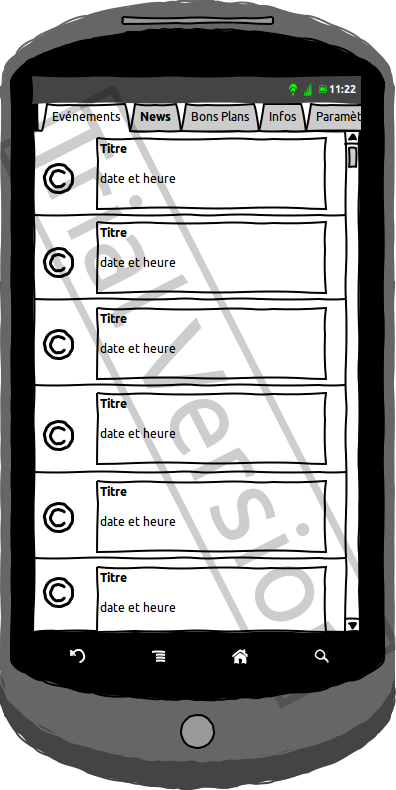
\includegraphics[scale=0.3]{../../Sketch/Android/News.png}
		\end{center}
	\end{minipage}
	\hfill
	\begin{minipage}[c]{.50\linewidth}
		\begin{center}
			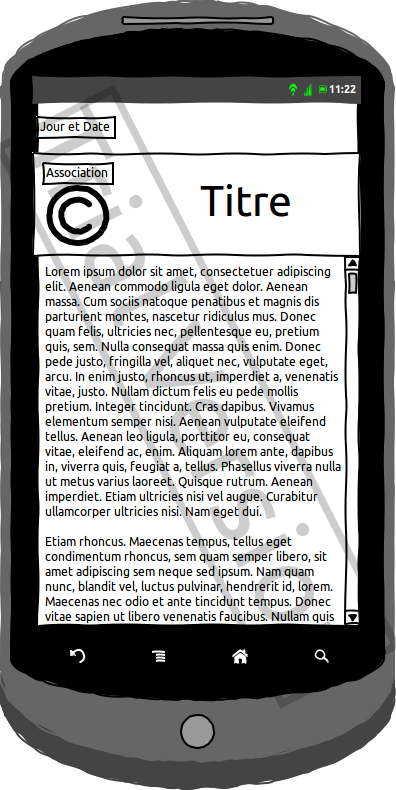
\includegraphics[scale=0.3]{../../Sketch/Android/DescrNews.png}
		\end{center}
	\end{minipage}
\end{figure}

\subsubsection{Pages bons plans}
Dans cette section, l'onglet actif est l'onglet "Bons plans".
\begin{figure}[htbp]
	\begin{minipage}[c]{.50\linewidth}
		\begin{center}
			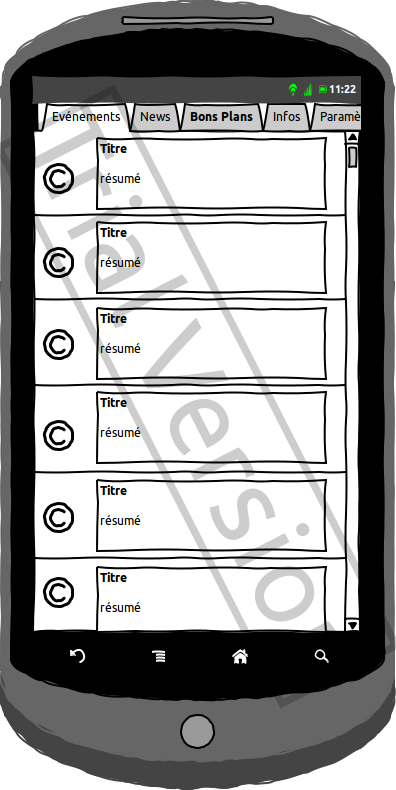
\includegraphics[scale=0.3]{../../Sketch/Android/BP.png}
		\end{center}
	\end{minipage}
	\hfill
	\begin{minipage}[c]{.50\linewidth}
		\begin{center}
			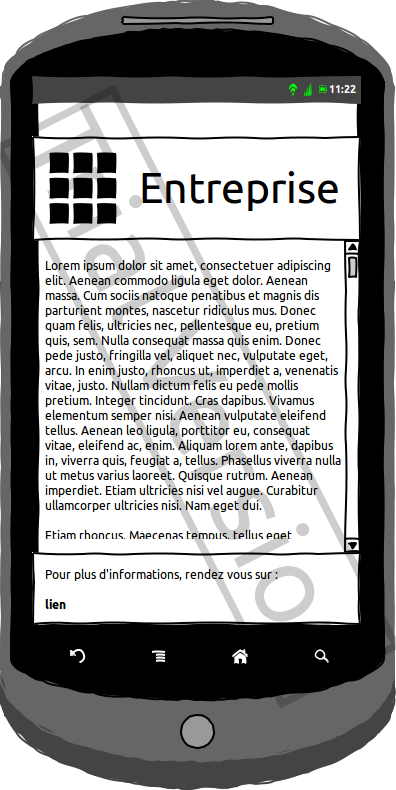
\includegraphics[scale=0.3]{../../Sketch/Android/DescrBP.png}
		\end{center}
	\end{minipage}
\end{figure}
\vfill
\clearpage

\subsubsection{Page informations}
Dans cette section, l'onglet actif est l'onglet "Infos".
La page information présente sur la même page deux liens cliquables et une description du Grand Cercle de Grenoble INP.
\vfill
\begin{figure}[htbp]
	\begin{minipage}[c]{.50\linewidth}
		\begin{center}
			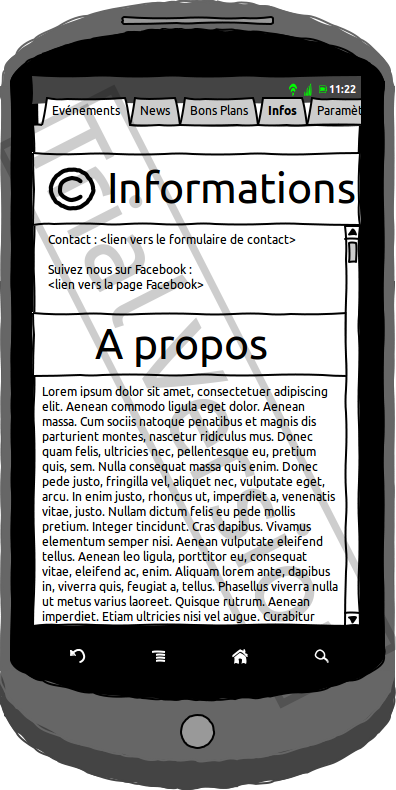
\includegraphics[scale=0.3]{../../Sketch/Android/Infos.png}
		\end{center}
	\end{minipage}
\end{figure}

\subsubsection{Pages paramètres}
Dans cette section, l'onglet actif est l'onglet "Paramètres". 
Pour sauvegarder ses préférences, il est nécessaire d'appuyer sur le bouton "OK" avant de quitter la fenêtre. La sauvegarde est effectuée au moment de l'appui sur ce bouton
\begin{figure}[htbp]
	\begin{minipage}[c]{.33\linewidth}
		\begin{center}
			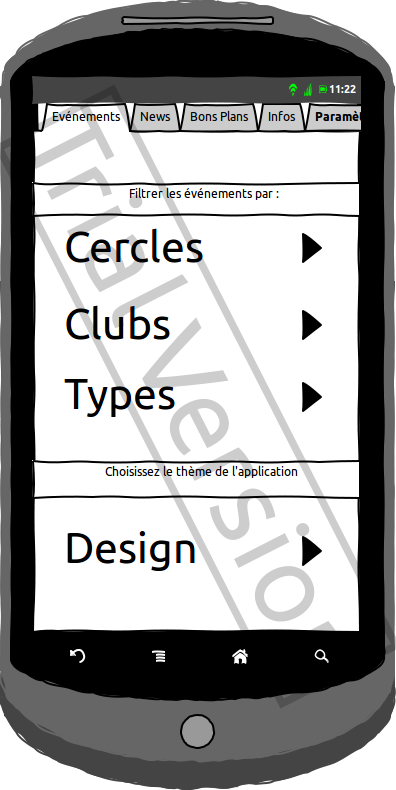
\includegraphics[scale=0.3]{../../Sketch/Android/Param.png}
		\end{center}
	\end{minipage}
	\hfill
	\begin{minipage}[c]{.33\linewidth}
		\begin{center}
			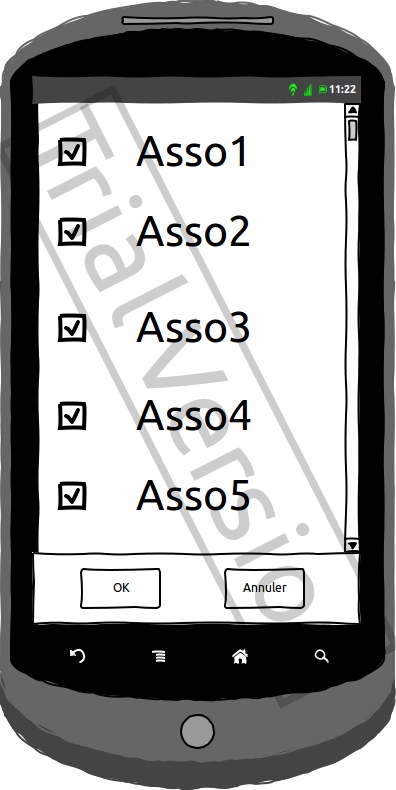
\includegraphics[scale=0.3]{../../Sketch/Android/Filtre.png}
		\end{center}
	\end{minipage}
	\hfill
	\begin{minipage}[c]{.32\linewidth}
		\begin{center}
			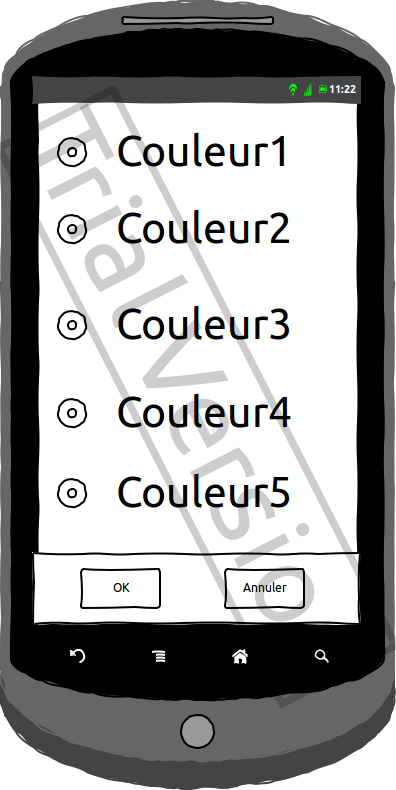
\includegraphics[scale=0.3]{../../Sketch/Android/Design.png}
		\end{center}
	\end{minipage}
\end{figure}
\vfill
\clearpage


\end{document}

